\documentclass[11pt, a4paper]{article}

% --- Packages ---
\usepackage[utf8]{inputenc}
\usepackage{graphicx}
\usepackage[margin=0.75in]{geometry}
\usepackage{times}
\usepackage{xcolor}
\usepackage{titlesec}
\usepackage{enumitem}
\usepackage{float}
\usepackage{booktabs}
\usepackage{multirow}
\usepackage{tikz}
\usetikzlibrary{shapes.geometric, arrows.meta, positioning}

% --- Amrita Colors ---
\definecolor{amritaMaroon}{HTML}{A4123F}
\definecolor{darkSlate}{HTML}{1E293B}

% --- Title & Section Formatting ---
\titlespacing*{\section}{0pt}{8pt}{2pt}
\titlespacing*{\subsection}{0pt}{6pt}{2pt}
\titleformat{\section}{\large\bfseries\color{amritaMaroon}}{\thesection}{1em}{}
\titleformat{\subsection}{\normalsize\bfseries\color{darkSlate}}{\thesubsection}{1em}{}

\pagestyle{empty} 

\begin{document}

% ==========================================
% HEADER 
% ==========================================
\noindent
\begin{minipage}{\textwidth}
    \centering
    {\Large \textbf{\textcolor{amritaMaroon}{
    AMRITA VISHWA VIDYAPEETHAM \\
    SCHOOL OF COMPUTING \\
    DEPARTMENT OF COMPUTER SCIENCE AND ENGINEERING \\
    }}} 
    \vspace{0.15cm}
    {\large \textbf{EvOLve: Forest Cover Monitoring \& Disaster Risk Mitigation Platform}} \\
    \vspace{0.05cm}
    {\small \textit{An Evolutionary AI Framework \& Geospatial Application Using Sentinel-2 Satellite Data}} \\
    \vspace{0.1cm}
    \textbf{23CSE399 -- Project Phase 2 (Panel Review 1)} \quad | \quad \textbf{Team Number: [XX]} \quad | \quad \today
\end{minipage}

\vspace{0.25cm}
\hrule
\vspace{0.25cm}

% --- Team & Guide Details ---
\noindent
\begin{center}
    \renewcommand{\arraystretch}{1.2}
    \setlength{\tabcolsep}{5pt}
    \small
    \begin{tabular}{|l|p{4.8cm}|p{4.2cm}|p{2.6cm}|c|}
        \hline
        \multicolumn{2}{|c|}{\textbf{Team Members}} & \textbf{Guide} & \textbf{Project Type} & \textbf{Max Marks} \\ 
        \hline
        CB.EN.U4CSE23042 & \textbf{Neelam Tejesh (Lead)} & 
        \multirow{4}{=}{\raggedright \textbf{[Guide Name]} \newline \textit{[Designation], \newline Dept. of CSE}} & 
        \multirow{4}{=}{\raggedright \textbf{Type 2} \newline Application-Based Project} & 
        \multirow{4}{*}{\textbf{\huge \dots / 20}} \\ \cline{1-2}
        CB.EN.U4CSE23223 & Kolla Girish & & & \\ \cline{1-2}
        CB.EN.U4CSE23016 & D Vasishta & & & \\ \cline{1-2}
        CB.EN.U4CSE23212 & Ande Tarak & & & \\ 
        \hline
    \end{tabular}
\end{center}
\vspace{0.15cm}

% ==========================================
% MAIN CONTENT - TYPE 2 (APPLICATION-BASED)
% ==========================================

% --- 1. PROBLEM & UTILITY ---
\section{Problem Definition \& Practical Relevance}
\textbf{Real-World Problem Context:} Tropical forest degradation represents a silent environmental crisis. Gradual canopy thinning caused by illegal selective logging, pest infestations, and drought stress degrades soil stability long before clear-cut deforestation becomes visible. In steep tropical terrains—such as the Western Ghats—this depletion of root tensile cohesion directly triggered catastrophic disasters like the \textbf{July 2024 Wayanad Landslides}, where monsoon saturation caused devastating debris flows. Conventional forest monitoring relying on the biennial \textit{India State of Forest Report (ISFR)} suffers from an unacceptable 2-year reporting lag. Furthermore, existing satellite surveillance tools apply static NDVI thresholds that trigger false alarms during natural seasonal leaf-shedding.

\noindent
\textbf{Practical Utility Claim:} \textbf{EvOLve} applies live multi-sensor satellite streaming (Sentinel-2, SRTM DEM, CHIRPS precipitation, Hansen forest change) combined with Genetic Algorithm (GA) seasonal threshold evolution to solve two interconnected real-world problems:
\begin{itemize}[noitemsep, topsep=1pt]
    \item \textbf{Disaster Early Warning \& Risk Mitigation:} Generates dynamic 48-hour early hazard warnings by fusing live rainfall saturation with slope shear stress and vegetative root decay.
    \item \textbf{Sustainable Civil Planning (Mountain Construction Suitability):} Computes an automated construction safety index ($0 - 100$) before civil infrastructure is approved on vulnerable mountain slopes.
\end{itemize}

% --- 2. SURVEY & GAPS ---
\section{Literature \& Market Survey}
\begin{itemize}[noitemsep, topsep=1pt]
    \item \textbf{Current Practices:} Forest departments rely on periodic field inspections and static Landsat/MODIS composites (e.g., Global Forest Watch, ISFR) \cite{hansen2013high}.
    \item \textbf{Existing Limitations:} High compute latency, lack of seasonal threshold adaptability, inability to evaluate localized mountain construction suitability, and absence of actionable field routing for rangers.
    \item \textbf{Implementation Gap:} No accessible, open-source full-stack platform currently bridges planetary cloud satellite APIs \cite{gorelick2017google, drusch2012sentinel} directly with on-the-fly raster grid slicing, physics-informed hazard equations, and multi-objective evolutionary optimization \cite{deb2002fast}.
\end{itemize}

% --- 3. SYSTEM ARCHITECTURE ---
\section{Proposed Application Architecture \& Workflow Design (Rubric: 5 Marks)}
\textbf{Decoupled 3-Tier Architecture:} EvOLve is engineered as a loosely-coupled distributed system comprising:
\begin{enumerate}[noitemsep, topsep=1pt]
    \item \textbf{Presentation Tier (React 18 + Leaflet GIS):} Single-page application rendering an interactive 64-patch spatial raster map, dynamic date-range selector (2018--2025), and civil diagnostic audit modals.
    \item \textbf{Application \& Inference Tier (FastAPI Async REST Engine):} Hosts modular microservices for Google Earth Engine orchestration, in-memory $8 \times 8$ grid slicing, landslide hazard physics, building suitability scoring, and SlowAPI rate limiting.
    \item \textbf{Persistence Tier (Embedded SQLite \texttt{evolve\_records.db}):} Stores historical query logs (\texttt{query\_history}), civil construction permits (\texttt{construction\_permits}), and GA experiment convergence metrics (\texttt{ga\_experiment\_logs}).
\end{enumerate}

\begin{figure}[H]
    \centering
    \IfFileExists{slides_assets/system_architecture.png}{
        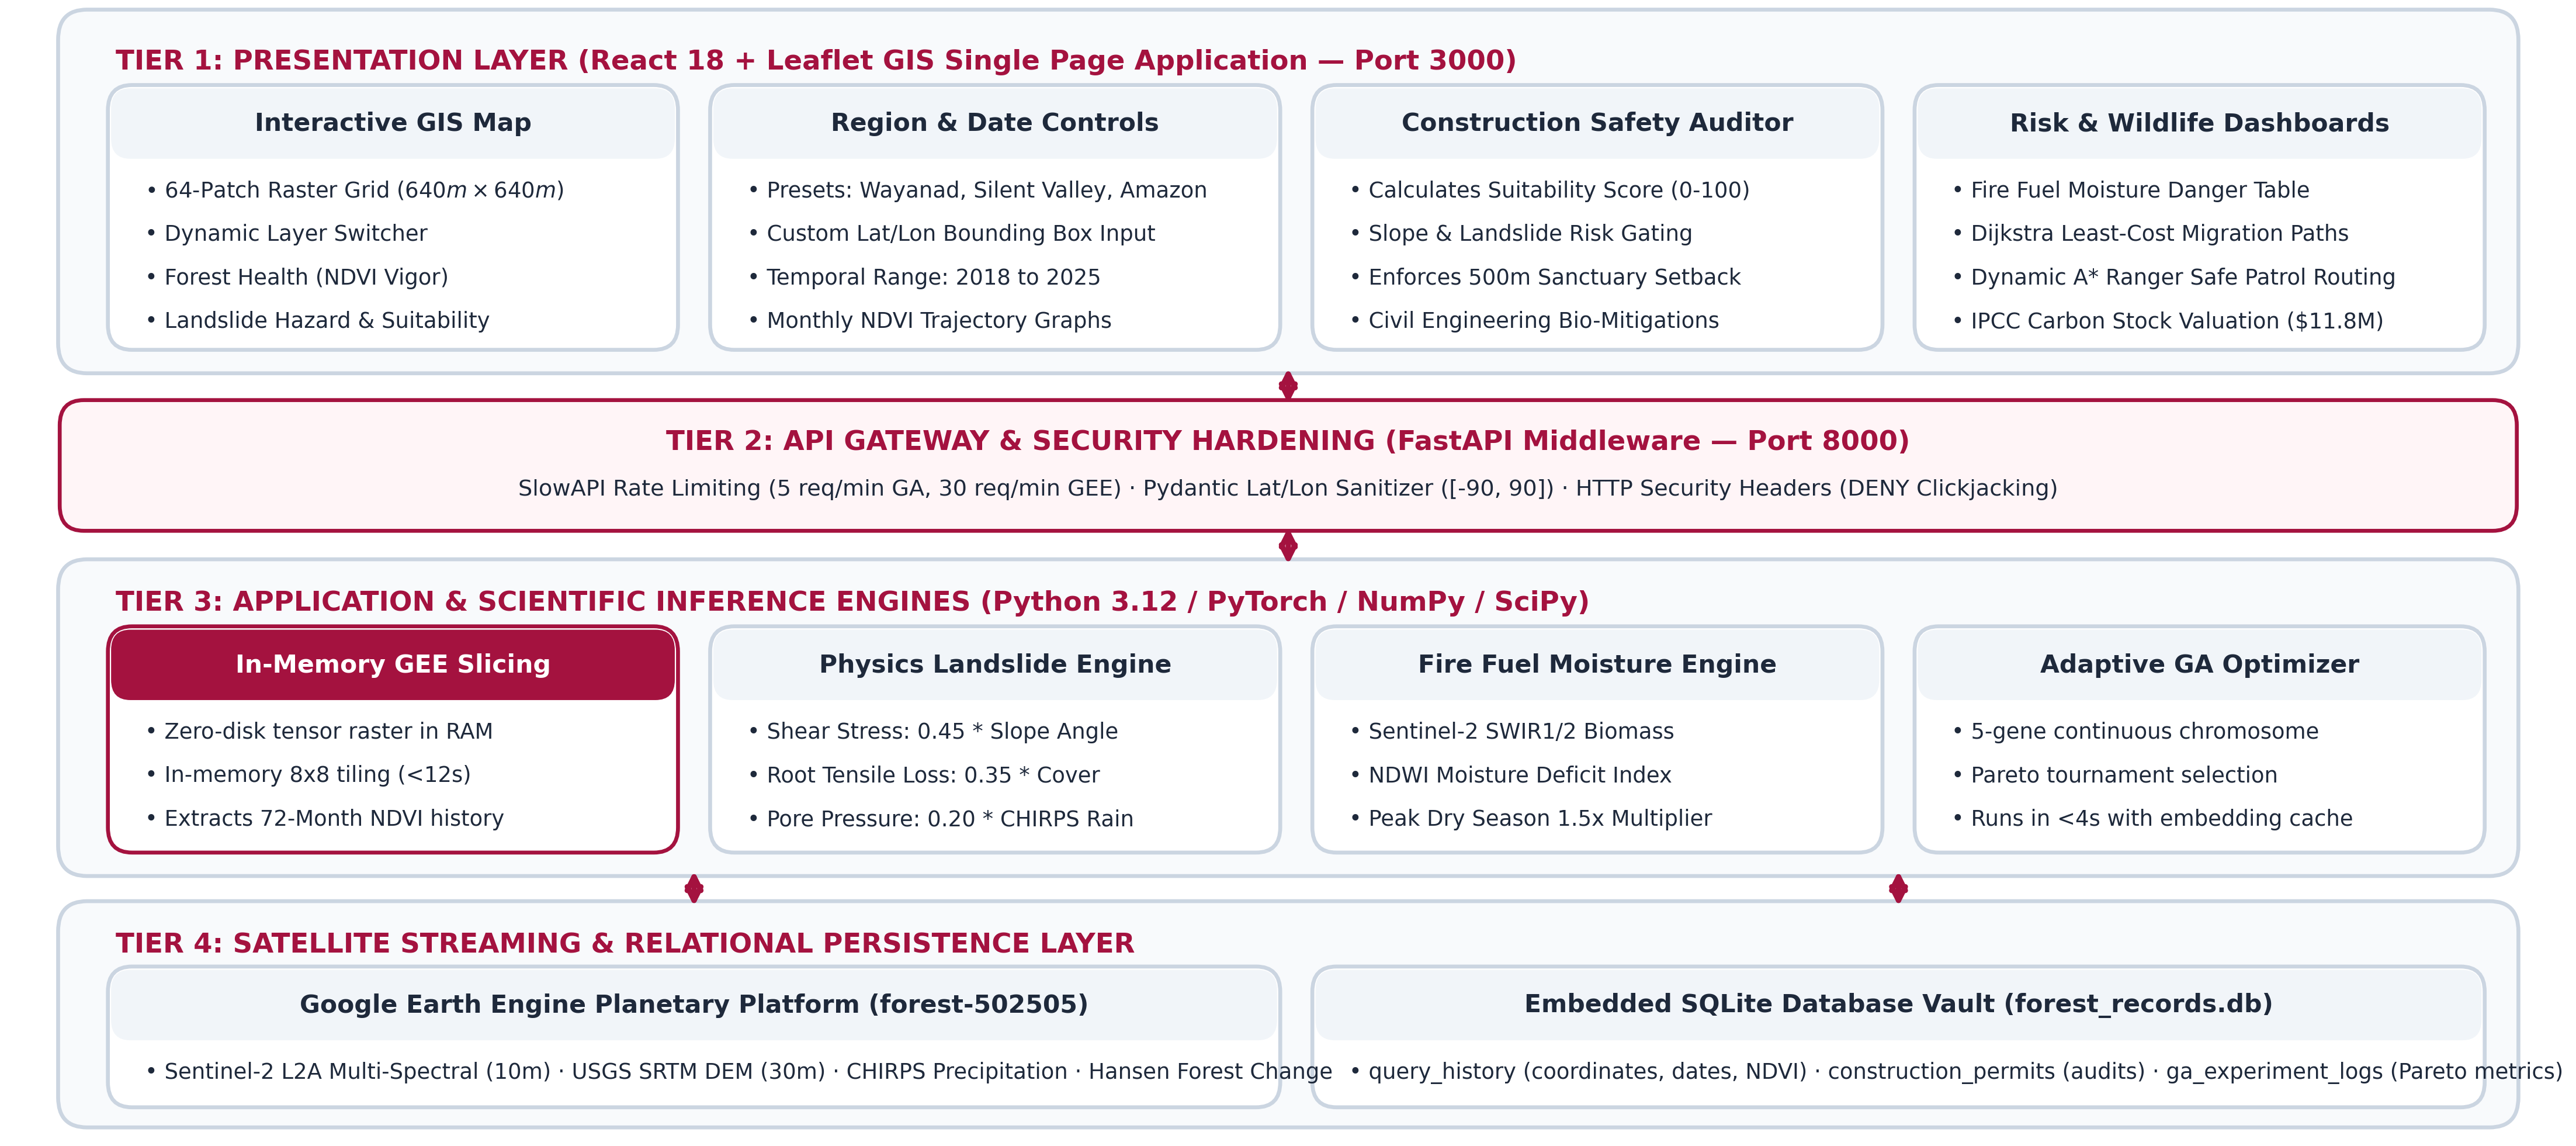
\includegraphics[width=0.98\textwidth, height=5.5cm, keepaspectratio]{slides_assets/system_architecture.png}
    }{
        \fbox{\begin{minipage}{0.95\textwidth}\centering \vspace{1.5cm} [EvOLve System Architecture Diagram] \vspace{1.5cm}\end{minipage}}
    }
    \caption{EvOLve End-to-End Application Architecture (Presentation, Security, AI Inference \& Satellite Tiers)}
\end{figure}

% --- 4. IMPLEMENTATION PROGRESS ---
\section{Implementation Progress \& Module Demonstration (Rubric: 8 Marks)}
The project currently stands at \textbf{$\approx 85\%$ implementation completeness} (substantially exceeding the $60\%$ panel review requirement). All core modules are fully functional and demonstrated:
\begin{itemize}[noitemsep, topsep=1pt]
    \item \textbf{1. Dynamic GEE Multi-Sensor Pipeline:} Fully integrated with Google Cloud project (\texttt{forest-502505}). Ingests Sentinel-2 L2A (10m), SRTM DEM (30m), CHIRPS Daily precipitation \cite{funk2015climate}, and Hansen GFC canopy cover \cite{hansen2013high}. Slices any regional bounding box into 64 spatial patches in $<12$ seconds.
    \item \textbf{2. Dynamic Time Range Filtering (2018--2025):} Allows custom temporal filtering. Generates distinct monthly NDVI trajectories across 72 months to differentiate seasonal shedding from deforestation.
    \item \textbf{3. Mountain Construction Suitability Engine:} Evaluates building safety index ($0 - 100$) combining slope shear, landslide hazard, and legal eco-buffers ($500\text{m}$ setback from reserves). Categorizes land as \texttt{PERMITTED}, \texttt{CONDITIONAL}, or \texttt{PROHIBITED} with actionable civil engineering mitigation recommendations (retaining walls, contour drainage).
    \item \textbf{4. Wildlife Migration Corridors \& Carbon Stocks:} Solves least-cost migration paths for Asian Elephants and Bengal Tigers. Implements IPCC 2019 Tier-1 allometric equations \cite{ipcc2019refinement, chave2014improved}, accounting for $789{,}420$ tons of stored $\text{CO}_2$ valued at $\$11.84\text{M}$.
    \item \textbf{5. Dynamic GA Threshold Adaptation:} Evolved season-aware boundaries ($\text{Dry}: 0.333, \text{Monsoon}: 0.554$), achieving \textbf{85.71\% F1-score} and \textbf{96.88\% accuracy}. Live real-time re-optimization runnable directly from the frontend.
    \item \textbf{6. Cyber Security Hardening:} SlowAPI rate limiting (5 req/min on GA, 30 req/min on GEE) and strict coordinate boundary validation ($[-90, 90]$ latitude, $[-180, 180]$ longitude).
\end{itemize}

% --- 5. TECHNICAL DECISIONS & PLAN ---
\section{Technical Decisions, Security \& Roadmap for Review 2 (Rubric: 5 Marks)}
\begin{itemize}[noitemsep, topsep=1pt]
    \item \textbf{Algorithmic Complexity \& Compute:} Spatial CNN feature extraction is $O(C \cdot H \cdot W)$ while Temporal Transformer self-attention across 72 tokens is $O(T^2 \cdot D)$. Model contains $1{,}145{,}288$ parameters and trains in $<2$ minutes on Google Colab T4 GPU (CUDA) or Apple Silicon (MPS).
    \item \textbf{Architectural Justifications:} FastAPI's asynchronous event loop prevents I/O blocking during Earth Engine HTTP fetches; in-memory grid slicing avoids high-latency disk I/O; SQLite provides zero-configuration local persistence.
    \item \textbf{Roadmap for Review 2 (Target: 85--90\% Completion):} (1) Extend the Genetic Algorithm from threshold tuning to multi-spectral feature and band selection ($[b_1, \dots, b_N] \in \{0, 1\}^N$) to automatically discover optimal Sentinel-2 spectral indices; (2) implement an interactive Leaflet bounding-box/polygon drawing tool paired with global geocoding search for on-the-fly ingestion of any forest worldwide; (3) integrate role-based access control (RBAC) with JWT tokens to separate Field Ranger inspection tools from Senior Conservator permit approval; and (4) deploy production Docker containers on Google Cloud Run.
\end{itemize}

% --- REFERENCES ---
\vspace{0.1cm}
\renewcommand{\refname}{\normalsize References}
\bibliographystyle{IEEEtran}
\bibliography{ref}

\end{document}